% 1. Presentación del problema de infiltración de agua
% 1.1 Ventajas de la simulación % Arley ayuda, sin tantas ecuaciones.
% Optimizar el uso del agua en el suelo, lograr el mayor contacto entre las capas periféricas de la raíz del suelo. 1 gota de aceite contamina un litro de agua. riego por surco, problema del percolación, los nutrientes son llevados, ejemplo con el café tradicional. problema
% cantidad desmedida de agua porque el suelo pierde sus nutrientes, %60% de eficiencia
% ejemplo de la caña: pesticidas, exceso de agua, etc (ciclo).
% el perder agua es mucho más caro para la humanidad.
% aportar a la agricultura de precisión
% ruta apoplástica (explica la interacción de la raíz agua)
% % el efecto de las algas (dia/noche) se puede explicar con el cloropasto () y la mitocondria (respiración)
% qué solución hay.
% de lo general a particular.
% [1] Ref.
\section{Presentation of water infiltration problem}
\subsection{Importancia}
\subsection{Justificación}
\subsection{Descripción del problema}
\begin{frame}
	\frametitle{\secname}
	\begin{minipage}{0.5\textwidth}
		\begin{itemize}
			\item .
		\end{itemize}
	\end{minipage}
	\begin{minipage}{0.47\textwidth}
		\begin{figure}[ht!]
			\centering
			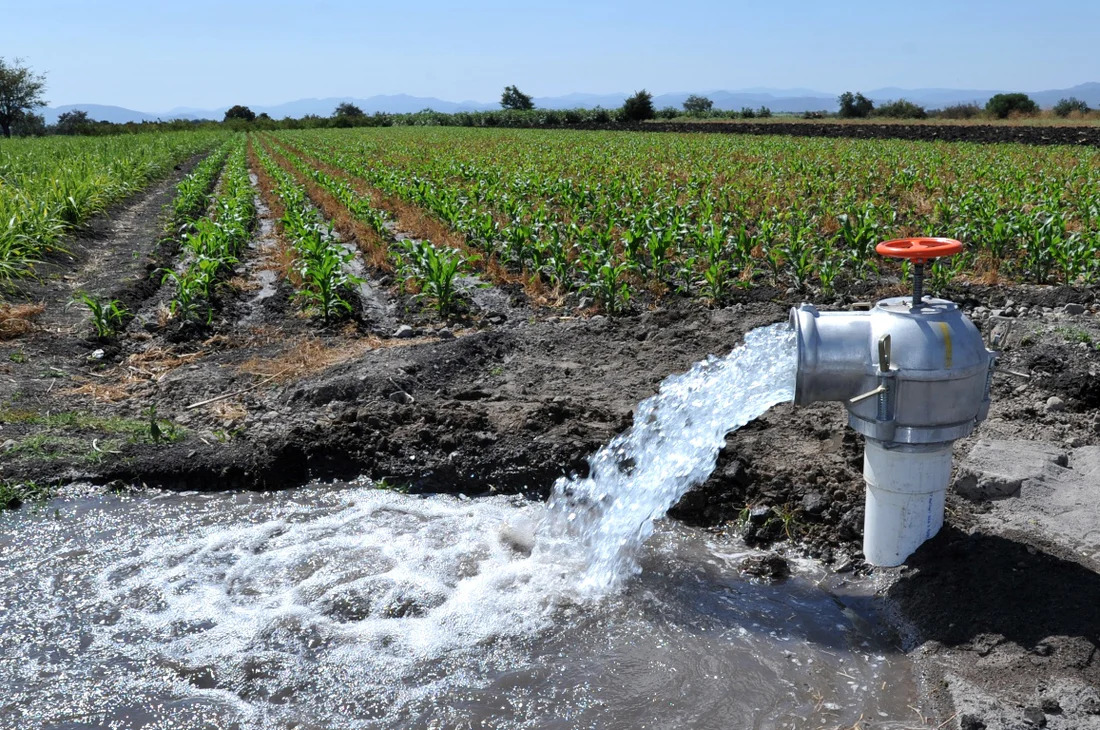
\includegraphics[height=5.5cm]{wasted_water}
			% https://proain.com/blogs/notas-tecnicas/calidad-del-agua-para-riego-agricola
		\end{figure}
	\end{minipage}
\end{frame}

\begin{frame}
	\frametitle{\secname}
	\begin{minipage}{0.5\textwidth}
		\begin{itemize}
			\item .
		\end{itemize}
	\end{minipage}
	\begin{minipage}{0.47\textwidth}
		\begin{figure}[ht!]
			\centering
			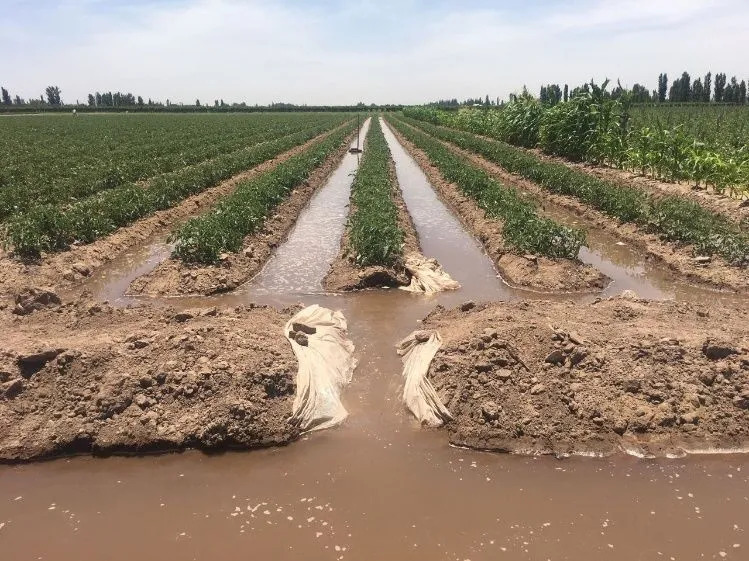
\includegraphics[height=5.5cm]{water_waster2}
			% https://www.agromeat.com/284499/conceptos-tecnicas-y-estrategias-en-uso-eficiente-del-agua-de-riego
		\end{figure}
	\end{minipage}
\end{frame}

% https://i.pinimg.com/originals/34/66/77/34667762422298ffc10fec5252f28619.jpg
\begin{frame}
	\frametitle{\secname}
	\begin{minipage}{0.47\textwidth}
		\begin{figure}[ht!]
			\centering
			\href{https://www.uneditorial.com/las-matematicas-en-la-vida-real-introduccion-basica-el-modelamiento-matematico-matematica.html}{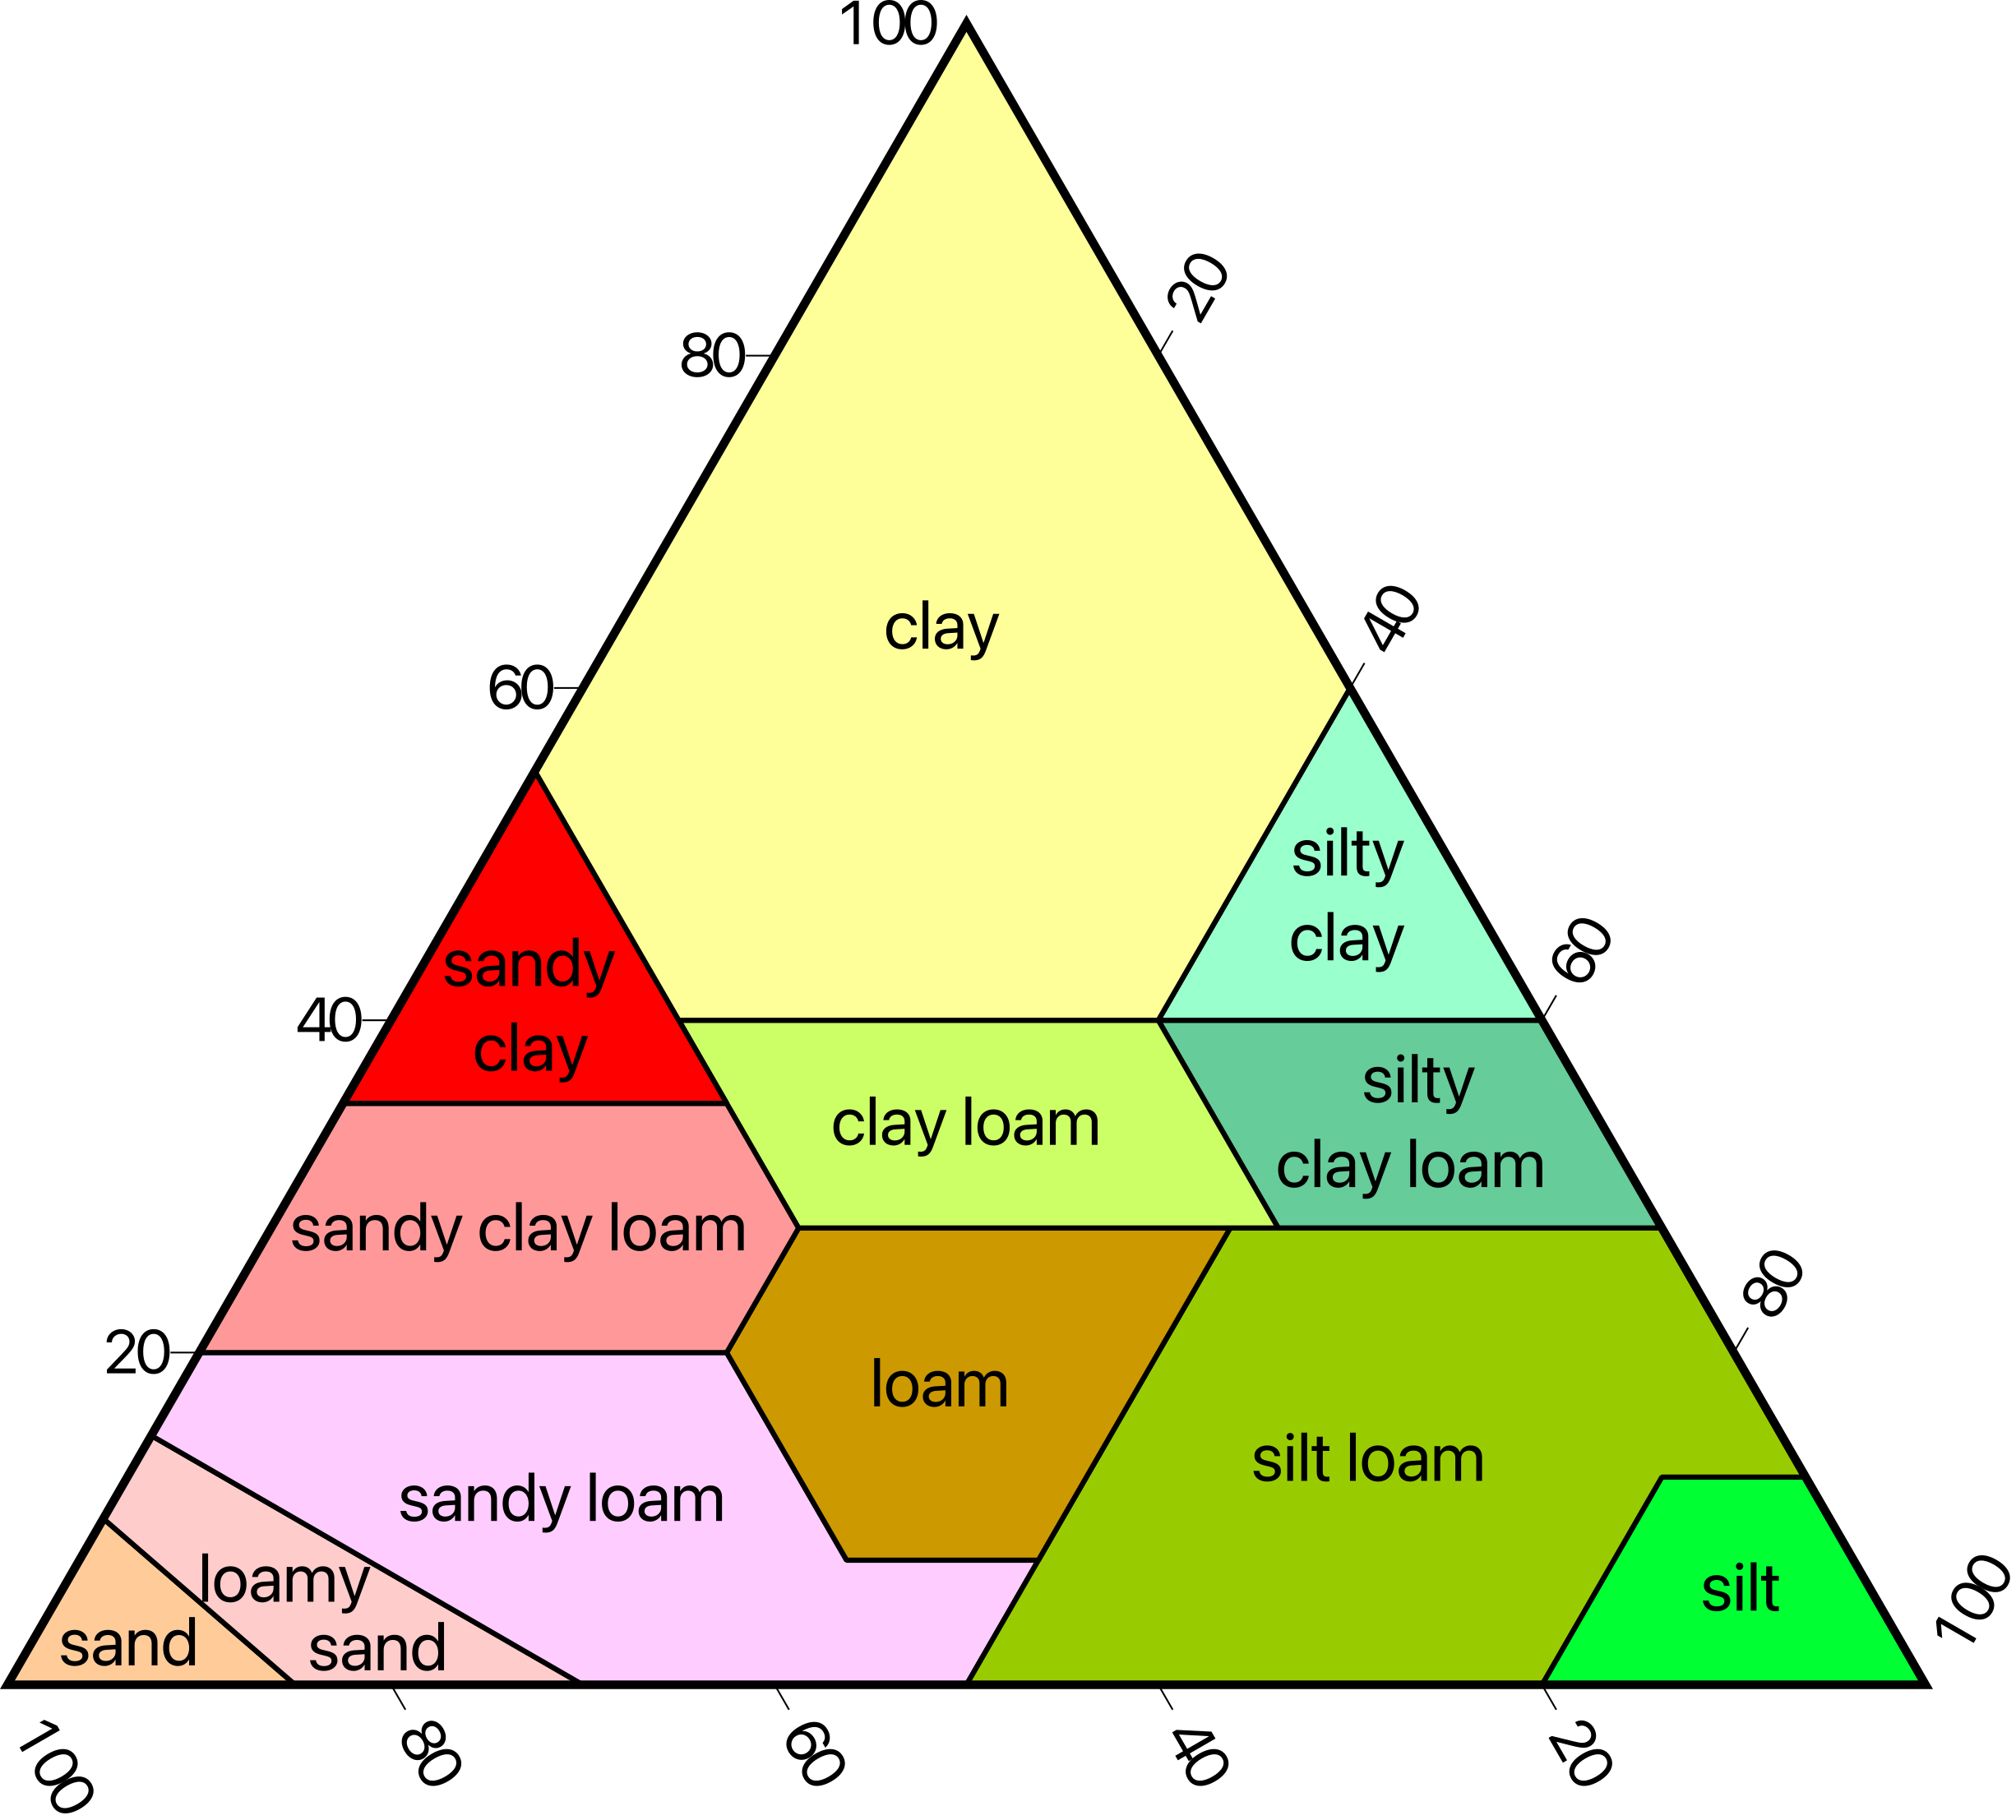
\includegraphics[height=5.5cm]{textural_soil}}
		\end{figure}
		\note{
			Los autores, John Jairo Leal y Juan Pablo Cardona les
			compartimos nuestro texto, y les contamos que es el producto
			de varios proyectos educativos de modelamiento matemático en
			las aulas en cursos de ingeniería.

			Una de nuestras líneas de investigación es precisamente la
			educación matemática para ingeniería y lo que esperamos es que
			más personas y más profesionales se vinculen con aplicaciones
			de matemáticas y con desarrollos futuros.
		}
	\end{minipage}
	\begin{minipage}{0.5\textwidth}
		\textsc{\Large Capítulos:}

		\

		\begin{enumerate}
			\item

			      Introducción a los números reales $\mathbb{R}$.

			      \

			\item

			      Introducción a las funciones.
		\end{enumerate}
	\end{minipage}
	\note{
		En su estructura el texto es introductorio para los primeros
		cursos de matemáticas, de hecho lo hemos utilizado en un curso
		que se llama matemáticas básicas, estudia las funciones y las
		derivadas y luego muestra algunos ejemplos de la vida cotidiana
		y cómo éstos se pueden escribir utilizando los símbolos
		matemáticos.
	}
\end{frame}

\begin{frame}
	\frametitle{\secname}
	\begin{figure}[ht!]
		\centering
		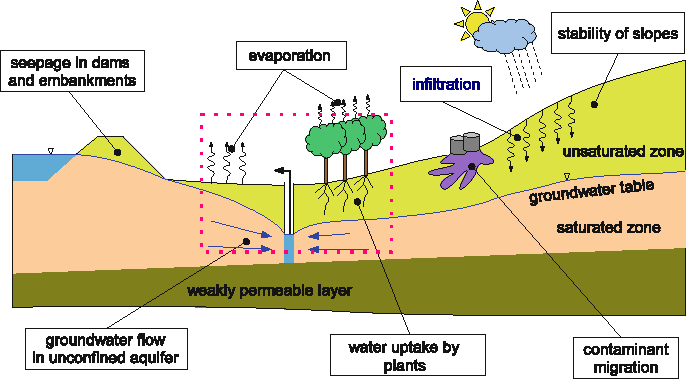
\includegraphics[height=6.8cm]{contamination}
	\end{figure}
	\note{
		En la diapositiva se muestra una de estas situaciones diarias.

		También se tiene un anexo donde se estudia un software libre
		como es \lstinline|wxmaxima|.
	}
\end{frame}
% Irricad

\begin{frame}
	\frametitle{\secname}
	\begin{figure}[ht!]
		\centering
		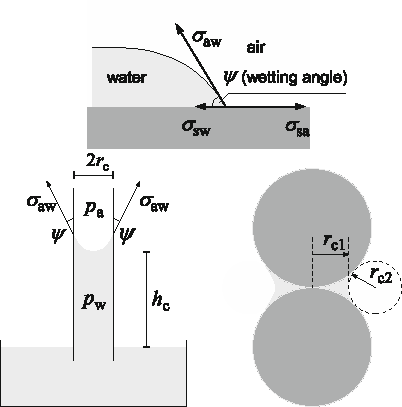
\includegraphics[height=6.8cm]{capillar_preassure}
	\end{figure}
\end{frame}

\begin{frame}
	\frametitle{\secname}
	\begin{figure}[ht!]
		\centering
		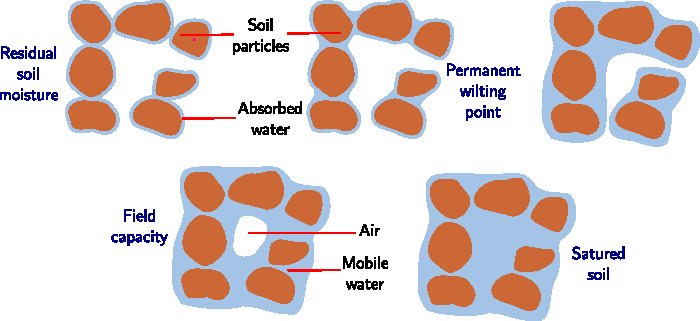
\includegraphics[height=6.8cm]{wetness}
	\end{figure}
\end{frame}